\documentclass{book}
\usepackage{graphicx} 
\usepackage[margin=2.5cm]{geometry}
\usepackage[italian]{babel}
\usepackage{amsmath}
\usepackage{amssymb}
\usepackage{amsthm}
\usepackage{hyperref}
\usepackage{xcolor}
\usepackage{tikz} % QUesto è per i Grafici 
\usetikzlibrary{arrows.meta,calc,positioning,decorations.pathreplacing}


\title{ELETTROMAGNETISMO: piselli, radiazioni e cazzi}
\author{NicoNico (PipoPipo), Michele Pisellini (michigay)}
\date{A.A. 2025/2026}


\begin{document}


\maketitle
\chapter*{Premessa}
     Non promettiamo rigore e assoluta correttezza nei seguenti appunti, visto che già è stato difficile cercare di seguire il buon Morgante ed i suoi giri pindarici durante le lezioni. Speriamo che tutto il nostro lavoro ed olio di gomito (stiamo copiando da appunti già esistenti e Griffiths) vi possano aiutare in questa materia, che tutt'ora non abbiamo capito se abbia o meno un ordine preciso, o se sia a libera interpretazione di chi la studia. 
    
    PS: non intendiamo in alcun modo seguire la sua notazione, ci teniamo alla vostra e sopratutto alla nostra saluta mentale. 


 

\[    
\underbrace{\lim_{t\to \infty} \text{percezione del tempo(t)} = \lim_{i\to \infty}\text{bestemmie}_i}_{\textbf{Legge Morgantica}} 
\]






\newpage
\tableofcontents

\newpage




\chapter{Introduzione matematica}
Riassumiamo in questa sezione gli strumenti matematici necessari in questo corso. Il consiglio spassionato che vi sentiamo di darvi è quello di fare Analisi 2 prima di Elettromagnetismo, fidatevi che vi si semplificheranno parecchie robe (anche perché ci rifiutiamo di rifare nei particolari tutta la parte sugli integrali della fisica che trovate comodamente sui pdf del corso di Sfecci).



\section{Flusso di un campo attraverso una superficie}
Prendiamo un generico campo vettoriale $\vec{C}$ ed una qualsiasi superficie S. Definiamo il flusso del campo attraverso la superficie come 
\begin{align*}
    \phi_{\vec{C}, S} = \int_S \vec{C}(\vec{r}) \cdot \hat{n} dS
\end{align*}

Se il campo considerato è uniforme, ossia ha sempre la stessa direzione, verso e modulo, e la superficie S è una superficie piana, abbiamo banalmente che
\begin{align*}
    \phi _{\vec{C}, S} = |\vec{C}| S \cos(\theta)
\end{align*}
dove $\theta$ è l'angolo che il campo forma con il versore della superficie. 

Nel caso in cui $S$ sia una superficie, il suo versore normale è positivo, orientato verso l'esterno e la notazione diventa
\begin{align*}
    \phi_{\vec{C}, S}= \oint_S \vec{C} (\vec{r})\cdot \hat{n}dS 
\end{align*}

Il "simbolo di vettore" sui campi, è proprio per dire che stiamo considerando delle funzioni vettoriali, cioè che prendono dei vettori e li mandano in altri vettori. Per quelli (sani) che preferiscono un pizzico di rigore matematico in più, stiamo semplicemente considerando delle funzioni
\begin{align*}
    F : \mathbb{R}^3\to \mathbb{R}^3
\end{align*}

In parole povere tutte le volte che parliamo di "campi", e vedete delle funzioni che hanno il simbolo di vettore sopra, stiamo prendendo la funzione appena scritta.
\section{Divergenza}
Definiamo la divergenza di un campo vettoriale nel seguente modo:
\begin{align*}
    \lim_{dV\to 0} \frac{\oint \vec{E}(\vec{r})\cdot \hat{n}dS}{dV} = \text{div} \vec{E}(\vec{r})
\end{align*}
dove $dV$ è il volume contenuto dalla superficie chiusa $dS$.
Prendiamo ora questa superficie e dividiamola in 2 parti. Il flusso di 1 su 2 e di 2 su 1 si annullano tra loro.
Possiamo considerare anche "infiniti" tagli su tutta la superficie, il che ci permette di ricavare 
\begin{align*}
    \int_{V_s} \text{div}\vec{C}(\vec{r}) dV = \int _{V_s} \left(\oint _S\vec{E}(\vec{r})\cdot \hat{n}dS \frac{1}{dV}\right) dV = \oint _S\vec{E}(\vec{r})\cdot \hat{n}dS
\end{align*}
che va sotto il nome di \textbf{teorema della divergenza}. Ovviamente questa non è in alcun modo una dimostrazione rigorosa di questo teorema, ma d'altronde siamo fisici e non matematici, perciò possiamo tranquillamente andare avanti.

Alcuni di voi si chiederanno, ma io ogni volta che devo ricavarmi la divergenza di un campo devo calcolarmi un integrale di superficie? La risposta è assolutamente no, anzi la formula per calcolare la divergenza è davvero molto molto semplice. Vediamo ora come ricavarla.
Vogliamo calcolare il flusso di un campo attraverso un cubo di volume infinitesimo $dV =dxdydz$.
Consideriamo la faccia $dydz$, la quale ha flusso $E_x(x+dx, y, z) dydz$, mentre la faccia opposta ha flusso $- E_x (x, y,z) dydz$. La somma dei due flussi ci da dunque come risultato 
\begin{align*}
    \left[ E_x(x+dx, y, z)- E_x(x,y,z)\right]dydz = \frac{\partial E_x}{\partial x} dx dy dz
\end{align*}
dove nell'uguaglianza abbiamo brutalmente moltiplicato e diviso per $dx$ (ricordo che siamo fisici e non matematici).
Ripetiamo questo procedimento per tutte le facce del cubo e sommiamo:
\begin{align*}
    \frac{\partial E_x}{\partial x}dxdydz+ \frac{\partial E_y}{\partial y}dxdydz + \frac{\partial E_z}{\partial z}dxdydz
\end{align*}
e dividiamo per $dV$:
\begin{align*}
\text{div} \vec{E}(\vec{r})= \frac{\partial E_x}{\partial x} + \frac{\partial E_y }{\partial y} + \frac{\partial E_z}{\partial z} = \vec{\nabla} \cdot \vec{E}
\end{align*}

\section{Gradiente, lavoro e campi conservativi}
Consideriamo adesso una funzione della sola posizione, ossia una funzione scalare $f(\vec{r})$. Premettiamo subito per i mathematical addicted che ora stiamo considerando funzioni del tipo 
\begin{align*}
    f: \mathbb{R}^3\to \mathbb{R}
\end{align*}
Definiamo il gradiente di $f$ come una quantità vettoriale che ci fornisce informazioni sulla direzione di massima variazione della funzione, e la ricaviamo come segue:
\begin{align*}
    f(\vec{r}+ d\vec{s}) - f(\vec{r}) = d\vec{s} \cdot \vec{\nabla }f (\vec{r}) = dx \frac{\partial f(\vec{r})}{\partial x}+ dy\frac{\partial f(\vec{r})}{\partial y}+ dz \frac{\partial f(\vec{r})}{\partial z}
\end{align*}
perciò il gradiente è il seguente vettore 
\begin{align*}
    \text{grad }f(\vec{r}) = \vec{\nabla}f(\vec{r}) = \left(\frac{\partial f(\vec{r})}{\partial x}, \frac{\partial f(\vec{r})}{\partial y}, \frac{\partial f(\vec{r})}{\partial z}\right)
\end{align*}

Infine, riprendiamo dalla dinamica la definizione di lavoro di una forza come integrale di linea:
\begin{align*}
    L = \int _a^b \vec{F} \cdot  d\vec{s}
\end{align*}
\section{Rotore}
Consideriamo le circuitazioni di un campo vettoriale su una qualsiasi curva chiusa $\gamma$, ossia
\begin{align*}
    \oint_{\gamma} \vec{E} \cdot d\vec{s}
\end{align*}
Se adesso dividiamo la curva in altre due $\gamma_1$ e $\gamma_2$, l'integrale di linea sarà la somma dei due integrali sulle due nuove curve. I contributi sulla linea dove abbiamo diviso il cammino originale saranno ovviamente nulli, dato che la percorriamo una volta in un senso e l'altra nell'altro.
Possiamo quindi suddividere il percorso in intervalli infinitesimali, ottenendo così:
\begin{align*}
    \hat{n}\cdot \text{rot} \vec{E} (\vec{r}) = \lim _{dS\to 0} \frac{\oint_{\gamma} \vec{E} \cdot d\vec{s}}{dS}
\end{align*}
dove $\hat{n}$ è il versore normale alla superficie.
Valutiamo ora come calcolare il rotore in coordinate cartesiane, considerando come prima un cubo di volume $dV = dxdydz$. Calcoliamo l'integrale di linea considerando i tratti opposti tra loro.
\begin{align*}
   &E_x (x,y,z)dx- E_x (x, y+dy, z) dx = [ E_x (x, y, z) - E_x (x, y+dy, z )] dx = - \frac{\partial E_x (x,y,z)}{\partial y} dy dx \\
   & E_y (x+ dx, y, z)dy - E_y(x, y, z)dy =[E_y (x+dx, y, z) - E_y (x, y, z)] dy = \frac{\partial E_y (x,y,z)}{\partial x} dxdy
\end{align*}
e perciò troviamo che 
\begin{align*}
     \text{rot} \vec{E} (\vec{r})|_{z}  =\frac{\partial E_y (x,y,z)}{\partial x} - \frac{\partial E_x (x,y,z)}{\partial y}
\end{align*}
Iteriamo questo procedimento anche per le altre componenti, ricavando 
\begin{align*}
    &\text{rot} \vec{E} (\vec{r})|_{x} = \frac{\partial E_z (x,y,z)}{\partial y} - \frac{\partial E_y (x,y,z)}{\partial z} \\
    &\text{rot} \vec{E} (\vec{r})|_{y} = \frac{\partial E_x (x,y,z)}{\partial z} - \frac{\partial E_z (x,y,z)}{\partial x}
\end{align*}

Abbiamo quindi trovato il rotore:
\begin{align*}
    \text{rot} \vec{E} = \vec{\nabla} \times \vec{E} = \left( \frac{\partial E_z}{\partial y}-\frac{\partial E_y}{\partial z}, \frac{\partial E_x}{\partial z}- \frac{\partial E_z}{\partial x}, \frac{\partial E_y}{\partial x}- \frac{\partial E_x}{\partial y} \right)
\end{align*}




















\chapter{Introduzione all'elettrostatica}
La materia possiede, oltre alla massa, una proprietà intrinseca detta carica elettrica, che dà luogo ad interazioni elettriche.  
L'elettrostatica studia queste interazioni sotto l'ipotesi ideale di condizioni stazionarie (cariche ferme).
Questa è un'approssimazione valida quando le cariche non si muovono o si muovono molto lentamente rispetto alle scale temporali di interesse.

\section{Legge di Coulomb}
La carica elettrica si presenta con due segni opposti (\emph{positivo} e \emph{negativo}). In molti materiali, su scala macroscopica, le cariche tendono a bilanciarsi (la materia è in genere elettricamente neutra), ma è possibile separare le cariche e creare distribuzioni con eccessi locali di carica. Le cariche producono campi elettrici e, in presenza di altre cariche, questi campi danno origine a forze elettriche. Tali forze, in genere, sono di gran lunga più intense delle forze gravitazionali a scale microscopiche.
\\
Dalle misure sperimentali compiute da Coulomb si ottiene la legge che esprime la forza elettrica che una carica puntiforme \(q_1\) esercita su un'altra carica puntiforme \(q_2\). La forma vettoriale della legge di Coulomb è
\[
\vec{{F}_{12}} 
= \frac{1}{4\pi\varepsilon_0}\;
\frac{q_1 q_2}{ \lvert{\vec{r}_2 - \vec{r}_1 } \rvert ^2} 
\underbrace{\frac{(\vec{r}_2 - \vec{r}_1 )}{\lvert{\vec{r}_2 - \vec{r}_1 } \rvert}}_{\text{versore}} 
= \frac{1}{4\pi\varepsilon_0}\;
\frac{q_1 q_2}{ \lvert{\vec{r}_2 - \vec{r}_1 } \rvert ^3} (\vec{r}_2 - \vec{r}_1 ),
\]


dove \(\mathbf r_1\) e \(\mathbf r_2\) sono le posizioni di \(q_1\) e \(q_2\) rispettivamente, e \(\varepsilon_0\) è la costante dielettrica del vuoto che vale: 
$$
\varepsilon_0= 8,85 \cdot 10^{-12} \frac{C^2}{N\cdot m^2}
$$
L'espressione per il modulo della forza, in funzione della distanza 

\(r=\lvert \vec{r}_2-\vec{r}_1\rvert\), è


\begin{figure}[ht]
  \centering
  \begin{minipage}[c]{0.7\textwidth} 
    \[
      F = \frac{1}{4\pi\varepsilon_0}\,\frac{\lvert q_1 q_2\rvert}{r^{2}}\hat{r}
    \]
  \end{minipage}\hfill
  \begin{minipage}[c]{0.28\textwidth}
    \begin{tikzpicture}[>=stealth, line width=0.9pt]

  \coordinate (A) at (0,0);
  \coordinate (B) at (2,1.25);

  \draw[->] (A) -- (B) node[midway, sloped, above] {$\mathit r$};
  
  \fill (A) circle (1.8pt) node[below left=2pt] {$q$};
  \fill (B) circle (1.8pt) node[above right=2pt] {$Q$};

\end{tikzpicture}
  \end{minipage}
\end{figure}


Il verso della forza dipende dai segni delle cariche: se i segni sono uguali la forza è repulsiva, se i segni sono opposti la forza è attrattiva.
Il modulo della forza $F_{q_{1}}$ è identico ad $F_{q_{2}}$ e l'unità di misura è Coulomb: $[F]= C$. Ovviamente per quanto detto prima questa legge vale solo per cariche ferme.


\subsection{Principio di sovrapposizione}
 Per un sistema di più cariche puntiformi $q_1, q_2 \dots, q_n $ alle distanze $r_1, r_2 \dots, r_n $  vale \textbf{il principio di sovrapposizione}: la forza totale su una carica $Q$ è la somma vettoriale delle forze dovute a ciascuna delle altre cariche.


\[
\vec{F_Q}=\sum_i \vec{F}_i = \vec{F}_1+\vec{F}_2+ \dots =  \frac{1}{4\pi\varepsilon_0}\,  ( \frac{ q_1 Q}{r_{1}^{2}} \hat{r_1} + \frac{ q_2 Q}{r_{2}^{2}}\hat{r_2}+\dots)
= \frac{Q}{4\pi\varepsilon_0}\, ( \frac{ q_1 }{r_{1}^{2}}\hat{r_1}+ \frac{ q_2 }{r_{2}^{2}}\hat{r_2}+\dots) 
\]   

\section{Il campo elettrico}
Dal Principio di sovrapposizione e legge di Coulomb siamo arrivati al seguente risultato che possiamo riscrivere in questo modo:
\[
\vec{F_Q}= \frac{Q}{4\pi\varepsilon_0}\,  \sum_i ( \frac{ q_i }{r_{i}^{2}}\hat{r_i}) = \frac{Q}{4\pi\varepsilon_0}\;
\sum_i \frac{q_i (\vec{r} - \vec{r}_i )}{ \lvert{\vec{r} - \vec{r}_i } \rvert ^3} 
\]
dove $\vec{E}(\vec{r}) \equiv \frac{1}{4\pi\varepsilon_0}\,  \sum_i ( \frac{ q_i }{r_{i}^{2}}\hat{r_i})$  viene definito come \textbf{Campo Elettrico}\footnote{Si sta facendo l'ipotesi di considerare un insieme discreto di cariche ferme }, si nota come questo è una funzione della posizione $\vec{r}$ siccome i vettori di separazione $\vec{r_i}$ dipendono dalla posizione del punto di campo.
Quindi il \textbf{Campo Elettrico} è una quantità vettoriale che varia da punto a punto ed è determinata dalla configurazione delle cariche sorgente.
Fisicamente è la forza che agisce su una carica unitaria dovuta a tutte le altre cariche presenti.
La sua unità di misura è $[E]=\frac{N}{C}$.

\begin{tikzpicture}[>=Stealth, font=\small]

  % ----------------------
  % Origine e punti (scelta per avere un ampio angolo O-S-P)
  % ----------------------
  \coordinate (O) at (0,0);         % origine
  \coordinate (S) at (3,4);         % source point (earlier was near the diagonal; now higher y)
  \coordinate (P) at (8,2);         % field point (further right, lower y than S) -> ampia area

  % ----------------------
  % Assi
  % ----------------------
  \draw[->, thin] (O) -- ++(10,0) node[right] {$x$};
  \draw[->, thin] (O) -- ++(0,6.5) node[above] {$y$};
  \draw[->, thin] (O) -- ++(-3.0,-2.4) node[below left] {$z$};
  \node[below left] at (O) {$0$};

  % ----------------------
  % Lati del triangolo (più spessi per risalto)
  % ----------------------
  \draw[->, line width=1.1pt] (O) -- node[pos=0.54, below] {$\mathbf r$} (P);       % O -> P
  \draw[->, line width=1.1pt] (O) -- node[pos=0.72, left] {$\mathbf r'_i$} (S);    % O -> S
  \draw[->, line width=1.1pt] (S) -- node[midway, above, sloped] {$\mathbf r_i$} (P);% S -> P

  % ----------------------
  % Vettore n_i breve (da S verso P ma visibile)
  % ----------------------
  \coordinate (midSP) at ($(S)!0.45!(P)$);
  \draw[->, line width=1.2pt] (S) -- ($(midSP)+(-0.40,0.25)$) node[midway, below right] {$\mathbf n_i$};

  % ----------------------
  % Punti ed etichette
  % ----------------------
  \fill (P) circle (2.6pt) node[above right] {Field point $P$};
  \fill (S) circle (2.2pt) node[above left,xshift=-2pt] {Source point};

  % ----------------------
  % Cluster di cariche intorno a S (distanziati)
  % ----------------------
  \foreach \dx/\dy/\lab in {-0.45/0.55/{$q_1$}, 0.22/0.40/{$q_2$}, -0.12/-0.35/{$q_i$}}{
    \coordinate (q) at ($(S)+(\dx,\dy)$);
    \fill (q) circle (1.6pt) node[shift={(0.18,0.08)}, font=\footnotesize] {\lab};
  }

  % ----------------------
  % Linee guida sottili (opzionali)
  % ----------------------
  \draw[thin, opacity=0.35] (O) -- (S) (S) -- (P);

\end{tikzpicture}

\subsection{Distribuzioni continue di cariche}
La definizione precedente di Campo Elettrico presupponeva che la sorgente del campo sia un insieme di cariche puntiformi discrete.
Se invece la carica è distribuita in modo continuo su una regione, allora il campo diventerà:

\[
\vec{E}(\vec{r})=\frac{1}{q}\int \vec{dF}(\vec{r})=  \frac{1}{4\pi\varepsilon_0} \int \frac{1}{r^2}\hat{r}dq
\]

Supponiamo ora di avere una distribuzione di carica volumetrica di carica ( e di non avere cariche esterne al di fuori del volume considerato).
Definiamo quindi la \textbf{densità volumetrica di carica} come $\rho(\vec{r})=\frac{dq}{dV} $
la cui dimensione è $[\rho]=\frac{C}{m^3}$.
Per quanto visto prima il Campo Elettrico (per una densità di carica volumetrica) sarà:

\[
\vec{E}(\vec{r})=\frac{1}{4\pi\varepsilon_0} \int_{V} \frac{(\vec{r} - \vec{r'} )}{ \lvert{\vec{r} - \vec{r'} } \rvert ^3}dq = \frac{1}{4\pi\varepsilon_0} \int_{V} \frac{(\vec{r} - \vec{r'} ) }{ \lvert{\vec{r} - \vec{r'} } \rvert ^3}\rho(\vec{r'}) dV
\]

Definiamo ora la \textbf{densità di carica superficiale} $\sigma$ \textbf{e lineare} $\lambda$ come: 
\[
\sigma(\vec{r}) = \frac{dq}{dS} 
\qquad 
[\rho] = \frac{C}{m^2}
\]
\[
\lambda(\vec{r}) = \frac{dq}{dl} 
\qquad 
[\rho] = \frac{C}{m}
\]

Con campi elettrici: 

\[
\vec{E}(\vec{r}) = \frac{1}{4\pi\varepsilon_0} \int_{S} \frac{(\vec{r} - \vec{r'} ) }{ \lvert{\vec{r} - \vec{r'} } \rvert ^3}\sigma(\vec{r'}) dS
\qquad 
\vec{E}(\vec{r}) = \frac{1}{4\pi\varepsilon_0} \int_{l} \frac{(\vec{r} - \vec{r'} ) }{ \lvert{\vec{r} - \vec{r'} } \rvert ^3}\lambda(\vec{r'}) dl
\]

\section{Esempi}


\chapter{Legge di Gauss}
\section{Linee di forza del campo elettrico}

Per rappresentare graficamente i campi elettrostatici e magnetici si utilizzano le \textbf{linee di campo} o \textbf{linee di forza}.  
Le \textbf{linee di forza} sono curve che, in ogni punto dello spazio, risultano tangenti al vettore campo. Su di esse si indica, mediante una freccia, il verso del campo stesso.  

\bigskip

\noindent
Consideriamo il \textbf{\textcolor{red}{caso 1}}, il più semplice possibile: una singola carica puntiforme $q$ posta nell’origine.  
Le linee di forza del campo avranno direzione radiale. Poiché il campo diminuisce come $\frac{1}{r^2}$, i vettori si accorciano man mano che ci si allontana dall’origine.  
L’intensità del campo non è indicata dalla lunghezza dei vettori, ma dalla \textbf{densità} delle linee di campo: il campo è più intenso dove le linee sono più ravvicinate (in prossimità dell’origine) e più debole dove esse si diradano.  

Anche se la rappresentazione avviene su una superficie bidimensionale, occorre ricordare che il campo possiede \textbf{simmetria sferica}.  
La densità delle linee può quindi essere espressa come:
\[
\frac{n}{S}
\]
dove $n$ è il numero di linee di campo e $S$ la superficie sulla quale esse si distribuiscono.  
\\
\\
Passiamo ora al \textbf{\textcolor{red}{caso 2}}: due cariche opposte disposte sullo stesso asse.  
Le linee di forza risultano perpendicolari al piano equatoriale e si estendono dalla carica positiva verso quella negativa.  
Sebbene le linee possano, in generale, estendersi all’infinito, in questo caso esse devono necessariamente chiudersi sulla carica opposta: se infatti considerassimo il flusso del campo attraverso una superficie chiusa che le racchiude, esso risulterebbe nullo, poiché il numero di linee che esce sarebbe uguale a quello che rientra.  

Inoltre, le linee di forza \textbf{non possono mai intersecarsi}, poiché ciò implicherebbe che in un punto il campo avesse due direzioni diverse, il che è fisicamente impossibile.  

Infine, se supponiamo che le due cariche siano poste a una distanza $r$ tra loro e che ci si trovi a una distanza $d \ll r$ da una delle due cariche $q_1$, l’effetto dell’altra carica $q_2$ diventa trascurabile, e il campo risulta praticamente quello di una singola carica.  
\\
\\
Vediamo ora il \textbf{\textcolor{red}{caso 3}}: due cariche uguali disposte sullo stesso asse.  
Lungo il piano equatoriale, il campo avrà una risultante parallela al piano stesso.  

È interessante notare che, allontanandosi molto dal sistema, la distanza tra le due cariche diventa trascurabile, al punto da non poter più distinguere se si tratta di due cariche o di una sola.  
In tal caso, le linee di forza delle due cariche tendono asintoticamente a configurarsi come linee di forza radiali che partono dal punto centrale tra le due cariche.  


\section{Legge di Gauss}
La \textbf{legge di Gauss} costituisce una delle relazioni fondamentali dell'elettrostatica e mette in relazione il flusso del campo elettrico attraverso una superficie chiusa con la carica elettrica racchiusa dalla superficie stessa. Essa è equivalente alle equazioni di Coulomb e di Maxwell in regime elettrostatico e rivela sia una interpretazione fisica del concetto di "sorgente" del campo elettrico sia uno strumento matematico potente per il calcolo del campo in presenza di opportune simmetrie.
Nel caso di una carica positiva avrò un flusso uscente (positivo), viceversa se è negativa; D'altra parte se ho una carica esterna alla superficie scelta, questa non contribuirà in alcun modo al flusso totale, poiché le sue linee di campo entrano da un lato ed escono dall'altro.
\\
\\
Consideriamo ora il \textbf{\textcolor{red}{caso 1}}: Flusso del campo elettrico di una carica puntiforme q, contenuta al centro di una sfera.

$$
\oint_{S}\vec{E}\cdot d\vec{S}
=\oint_{S}\vec{E}\cdot \hat{n}d{S}
=
\int_{0}^{2\pi} \int_{0}^{\pi}
\frac{1}{4\pi\varepsilon_0}\frac{q \hat{\mathbf r}}{r^{2}}
\bigl(r^{2}\sin\theta d\theta d\phi \hat{\mathbf r}\bigr)
=\int_{0}^{2\pi} \int_{0}^{\pi}\frac{q}{4\pi\varepsilon_0}\,\sin\theta d\theta d\phi= \frac{q}{\varepsilon_0}.
$$
Si osservi che la dipendenza dal raggio si annulla: l’area della sfera cresce come  $r^{2} $, mentre il campo elettrico diminuisce come $\frac{1}{r^{2}}$ ; il loro prodotto risulta quindi costante. Ne consegue che lo stesso numero di linee di campo attraversa qualsiasi sfera centrata nell’origine. In generale, il flusso attraverso una superficie chiusa dipende solo dalla carica racchiusa, indipendentemente dalla posizione della carica  e dalla forma e dimensioni della superficie.
Ciò che conta è l’angolo solido $d\Omega = \frac{dS\cos\theta}{r^{2}}$ che dovrà essere $\Omega=4\pi$. 
\\
\\
Vediamo il \textbf{\textcolor{red}{caso 2}}: Gruppo di cariche sparse all'interno della superficie.
Possiamo sfruttare il \textbf{Principio di sovrapposizione} e scrivere:

\[
\oint \vec{E} \cdot d\vec{S}
=  \oint \sum_{i=1}^{n}\vec{E}_i \cdot d\vec{S} 
= \sum_{i=1}^{n} \left( \oint \vec{E}_i \cdot d\vec{S} \right)
= \sum_{i=1}^{n} \left( \frac{1}{\varepsilon_0} q_i \right)=  \frac{Q_{int}}{\varepsilon_0}  
\]
Dove $Q_{int}$ è la carica interna alla superficie gaussiana considerata. 

\[
\boxed{
\oint \vec{E} \cdot d\vec{S}
= \frac{Q_{int}}{\varepsilon_0} 
}
\]



\subsection{Formulazione infinitesimale e I legge di Maxwell}
Supponiamo ora di avere una carica distribuita su un volume, sia $\rho(\vec{r})$ la densità volumetrica di carica, allora si ha:
$$
\oint_{S}\vec{E}\cdot \hat{n}d{S} = \frac{1}{\varepsilon_0}\int_{V_s} \rho(\vec{r})d{V}
$$
Possiamo sfruttare il teorema della divergenza e scrivere:
$$
\oint_{S} \vec{E} \cdot \hat{n}\, dS = \int_{V_s} (\vec{\nabla} \cdot \vec{E})\, dV = \frac{1}{\varepsilon_0}\int_{V_s} \rho(\vec{r})d{V}
$$
Essendo gli integrali sullo stesso volume si trova così la \textbf{I equazione di Maxwell o Legge di Gauss}, un equazione che lega la divergenza del campo elettrico alla densità di carica.
$$
\boxed{
\vec{\nabla} \cdot \vec{E} = \frac{1}{\varepsilon_0} \rho
}
$$

\section{Esempi}

\chapter{Il potenziale elettrico}
Vogliamo definire un potenziale scalare associato al campo elettrico.  
Per farlo, mostreremo che il campo elettrico è un campo irrotazionale, ovvero il suo rotore è nullo.  
Questo ci permetterà di introdurre il concetto di potenziale elettrico, grandezza scalare da cui è possibile ricavare il campo stesso.
\section{Il rotore di E}
Il campo elettrico $\vec{E}$ non è una funzione vettoriale qualsiasi, ma un tipo molto speciale di campo: uno il cui rotore è nullo.  
Sfrutteremo questa proprietà dei campi elettrostatici per ridurre un problema vettoriale (determinare $\vec{E}$) a un problema scalare molto più semplice.
\\
\\
Consideriamo l’integrale di linea lungo un percorso (da $a$ a $b$) del campo elettrico generato da una carica puntiforme:
\[
\int_a^b \vec{E}(\vec{r}) \cdot d\vec{l} 
= \int_a^b \frac{q}{4\pi \varepsilon_0 r^2} \hat{r} \cdot d\vec{l} 
\quad \text{con} \quad \hat{r} \cdot d\vec{l} = dr
\]
\[
= \frac{q}{4\pi \varepsilon_0} \int_a^b \frac{dr}{r^2} 
= \frac{q}{4\pi \varepsilon_0} \left( \frac{1}{r_a} - \frac{1}{r_b} \right)
\]
Da cui segue immediatamente che, se $r_a = r_b$, l’integrale di linea è nullo.  
Possiamo quindi affermare che, \textbf{per campi elettrostatici},
\[
\oint_{\gamma} \vec{E} \cdot d\vec{l} = 0
\]
e, in base al \textbf{teorema di Stokes} (o del rotore):
\[
\boxed{
\vec{\nabla} \times \vec{E} = 0
}
\]
Si deduce facilmente che anche nel caso in cui si abbiano $N$ cariche, anche con il principio di sovrapposizione, l’integrale di linea resta nullo per l’additività dell’integrale.  
Di conseguenza, il teorema di Stokes risulta valido anche in questo caso.

\section{Introduzione al potenziale}

Il \textbf{potenziale elettrico} \(V(\vec r)\) è una grandezza scalare che caratterizza un campo elettrostatico \(\vec{E}(\vec r)\).
Poiché, per un campo elettrostatico conservativo, l'integrale di linea è indipendente dal percorso (dipende solo dai punti iniziale e finale), si definisce
\[
\boxed{%
V(\vec{r}) \equiv - \int_{\mathcal{O}}^{\vec{r}} \vec{E}(\vec{r}\,') \cdot d\vec{l}
}
\]
dove \(\mathcal{O}\) è un punto di riferimento scelto (convenzionalmente il punto in cui si assegna \(V=0\)). Di conseguenza \(V\) dipende solo dalla posizione \(\vec r\).

Ciò che ha significato fisico è la differenza di potenziale tra due punti \(a\) e \(b\):
\[
\Delta V_{ab} = V(b)-V(a) = -\int_{a}^{b} \vec{E}\cdot d\vec{l}.
\]
Dal teorema fondamentale del calcolo (applicato lungo una curva) si ha inoltre
\[
V(b)-V(a)=\int_{a}^{b} (\nabla V)\cdot d\vec{l}.
\]
Poiché le due espressioni valgono per ogni coppia di punti \(a,b\), si ottiene la relazione locale
\[
\boxed{\vec{E}(\vec r) = -\,\nabla V(\vec r).}
\]

\subsection*{Commenti sul potenziale}

\begin{itemize}
  \item Utilizzare il potenziale risulterà spesso più semplice per determinare il campo elettrico.
  \item Il punto di riferimento \(\mathcal{O}\). Cambiare il punto di riferimento equivale ad aggiungere una costante \(C\) al potenziale. Infatti, scegliendo un altro riferimento \(\mathcal{O}'\),
    \[
      V'(\vec{r}) = - \int_{\mathcal{O}'}^{\vec{r}} \vec{E}\cdot d\vec{l}
      = -\int_{\mathcal{O}'}^{\mathcal{O}} \vec{E}\cdot d\vec{l} -\int_{\mathcal{O}}^{\vec{r}} \vec{E}\cdot d\vec{l}
      = V(\vec{r}) + C,
    \]
    dove \(C = -\displaystyle\int_{\mathcal{O}'}^{\mathcal{O}} \vec{E}\cdot d\vec{l}\). Naturalmente aggiungere una costante a \(V\) non modifica né le differenze di potenziale né il gradiente \(\nabla V\).
  \item Principio di sovrapposizione: se \(\vec{E}=\sum_{i=1}^N \vec{E}_i\), allora
    \[
      V(\vec r) = -\int_{\mathcal{O}}^{\vec r} \vec{E}\cdot d\vec l
               = -\int_{\mathcal{O}}^{\vec r}\sum_{i=1}^N\vec{E}_i\cdot d\vec l
               = \sum_{i=1}^N \left(-\int_{\mathcal{O}}^{\vec r}\vec{E}_i\cdot d\vec l\right)
               = \sum_{i=1}^N V_i(\vec r).
    \]
  \item Unità di misura: il potenziale si misura in Volt (V), dove
    \[
      [V] = \mathrm{V} = \frac{\mathrm{J}}{\mathrm{C}} = \frac{\mathrm{N\,m}}{\mathrm{C}}.
    \]
\end{itemize}

\section{Potenziale della carica puntiforme}

Per una carica puntiforme \(q\) posta nell'origine il campo elettrico è
\[
\vec{E}(\vec r)=\frac{1}{4\pi\varepsilon_0}\,\frac{q}{r^{2}}\hat r.
\]
Scegliendo come riferimento il potenziale nullo all'infinito (\(\mathcal{O}=\infty\)) si ha
\[
V(\vec r)= -\int_{\infty}^{r} \vec{E}\cdot d\vec l
= -\int_{\infty}^{r} \frac{q}{4\pi\varepsilon_0}\,\frac{1}{r'^{2}}\,dr'
= \frac{q}{4\pi\varepsilon_0}\,\frac{1}{r}.
\]
Quindi il potenziale di una carica puntiforme (con \(V(\infty)=0\)) è
\[
\boxed{\,V(\vec r)=\dfrac{q}{4\pi\varepsilon_0\,r}\,.}
\]

Ora, per un sistema discreto di \(N\) cariche puntiformi \(\{q_i\}\) distribuite nelle posizioni \(\{\vec r_i\}\), il principio di sovrapposizione afferma che il campo totale è la somma dei campi individuali:
\[
\vec{E}(\vec r)=\sum_{i=1}^N \vec{E}_i(\vec r).
\]
Ne segue che il potenziale totale, definito come
\[
V(\vec r) = -\int_{\infty}^{\vec r} \vec{E}(\vec r\,')\cdot d\vec l,
\]
si può scrivere come somma dei contributi individuali:

\[
\boxed{\,V(\vec r)=\sum_{i=1}^{N}\dfrac{q_i}{4\pi\varepsilon_0\,|\vec r-\vec r_i|}\, .}
\]

\section{Potenziale di una distribuzione uniforme di carica}

Calcoliamo il potenziale generato da una distribuzione volumetrica di carica. Conoscendo il potenziale di una carica puntiforme, si divide il volume in elementi infinitesimi di carica \(dq\) e si sommano (integrando) i contributi di tutte le parti:

\[
V(\vec{r}) = \frac{1}{4\pi\varepsilon_0}\int_{\mathcal{V}}\frac{1}{|\vec{r}-\vec{r}\,'|}\,dq.
\]

Ricordando che \(dq=\rho(\vec{r}\,')\,dV'\), si ottiene

\[
\boxed{%
V(\vec{r}) = \frac{1}{4\pi\varepsilon_0}\int_{\mathcal{V}}\frac{\rho(\vec{r}\,')}{|\vec{r}-\vec{r}\,'|}\,dV'
}
\]
dove \(\mathcal{V}\) indica il dominio volumetrico occupato dalla distribuzione di carica e \(\rho(\vec r\,')\) è la densità volumetrica di carica.


\section{Esempi}
\section{Equazione di Poisson}

Abbiamo trovato che il \textbf{campo elettrico} ($\vec{E}$) può essere scritto come il \textbf{gradiente} di una funzione scalare, il \textbf{potenziale elettrostatico} ($V$):
$$
\vec{E} = - \vec{\nabla} V
$$
mentre dalla \textbf{legge di Gauss} per il campo elettrico nel vuoto si ha:
$$
\vec{\nabla} \cdot \vec{E} = \frac{\rho}{\epsilon_0}
$$
dove $\rho$ è la densità di carica e $\epsilon_0$ è la permittività elettrica del vuoto.
Mettendole assieme (sostituendo la prima nella seconda) si ottiene:
$$
\vec{\nabla} \cdot (-\vec{\nabla} V) = \frac{\rho}{\epsilon_0}
$$
ovvero
$$
\nabla^2 V = - \frac{\rho}{\epsilon_0}
$$
Si trova quindi l'\textbf{Equazione di Poisson}, dove $\nabla^2 = \vec{\nabla} \cdot \vec{\nabla}$ è l'operatore \textbf{Laplaciano}.
Perciò, in una regione dove non ci sono cariche, la \textbf{densità di carica è nulla} ($\rho=0$), si ottiene:
$$
\nabla^2 V = 0
$$
Ottenendo l'\textbf{Equazione di Laplace}.

\section{Condizioni al contorno / Boundary conditions}
Determiniamo proprietà generali per il campo elettrico quando si attraversa una superficie che porta una densità di carica superficiale.
In un tipico problema elettrostatico viene fornita una distribuzione di carica sorgente $\rho$ e si desidera trovare il campo elettrico $\vec{E}$ che essa produce. A meno che la simmetria del problema non consenta una soluzione immediata tramite la legge di Gauss, è spesso conveniente calcolare prima il potenziale elettrico come passaggio intermedio.

\begin{itemize}
\item[\textbf{(1)}] \textbf{Componente normale (perpendicolare) -- discontinuità.}\\
Supponiamo che la superficie abbia \textbf{spessore nullo}.
Vogliamo capire cosa succede attraversando la superficie. Sappiamo che:
$$
\vec{\nabla}\cdot\vec{E}(\vec{r}) = \frac{\rho(\vec{r})}{\varepsilon_0},
\qquad 
\vec{\nabla}\times \vec{E} = 0.
$$

Consideriamo una \textbf{superficie gaussiana cilindrica} di altezza trascurabile ($h \to 0$). Poiché la regione è molto piccola, possiamo considerare $\vec{E}(\vec{r})$ costante. Si ha quindi:
$$
\oint \vec{E}\cdot \hat{n}\,dS 
= \underbrace{\int_{S_{lat}}\vec{E}_l\cdot \hat{n}\,dS}_{\text{($h \sim 0$) $\to 0$}} 
+ \int_{S_{b1}}\vec{E}_1\cdot \hat{n}\,dS 
+ \int_{S_{b2}}\vec{E}_2\cdot \hat{n}\,dS 
= \int_{S_{b1}}E_{\perp 1}\,dS - \int_{S_{b2}}E_{\perp 2}\,dS.
$$
Dove $S_{lat}$ è la superficie laterale del cilindro e $S_{b1}$, $S_{b2}$ le superfici di base. In uno dei due integrali compare un segno negativo perché il versore normale è opposto. Si ottiene quindi:
$$
E_1 S_b - E_2 S_b = \frac{Q}{\varepsilon_0} = \frac{\sigma S_b}{\varepsilon_0},
$$
e di conseguenza:
$$
E_{\perp 1} - E_{\perp 2} = \frac{\sigma}{\varepsilon_0}.
$$
Attraversando una qualsiasi superficie carica, la componente perpendicolare del campo elettrico presenta quindi una discontinuità pari a $\frac{\sigma}{\varepsilon_0}$.
\\
\\
\item[\textbf{(2)}] \textbf{Componente tangenziale (parallela) -- continuità.}\\
Per la componente parallela alla superficie, utilizziamo invece il fatto che il rotore del campo elettrico è nullo. 
Consideriamo un percorso rettangolare (una superficie di Stokes) con i lati lunghi paralleli alla superficie e quelli corti perpendicolari, in modo da poter trascurare il loro contributo poiché $h \sim 0$. 
Applicando la circuitazione del campo elettrico si ottiene:
$$
\oint \vec{E}\cdot d\vec{l} = 
\int_{l_1}\vec{E}_1\cdot d\vec{l} + \int_{l_2}\vec{E}_2\cdot d\vec{l} 
= \int_{l}E_{\parallel 1}\,dl - \int_{l}E_{\parallel 2}\,dl
= E_{\parallel 1}l - E_{\parallel 2}l.
$$
Ne segue che attraversando una qualunque superficie carica, la componente parallela del campo elettrico non presenta discontinuità:
$$
E_{\parallel 1} - E_{\parallel 2} = 0 \quad \Rightarrow \quad E_{\parallel 1} = E_{\parallel 2}.
$$
\
\end{itemize}

\subsection*{Verifiche su casi noti}
\begin{itemize}
  \item \textbf{Piano infinito carico:}\\
  Per un piano infinito con densità superficiale $\sigma$ il campo è uniforme da entrambi i lati e si verifica
  $$
  \Delta E_{\perp} = \frac{\sigma}{\varepsilon_0}, \qquad \Delta E_{\parallel} = 0.
  $$
  \item \textbf{Due piani con cariche opposte:}\\
  Anche in questo caso valgono le stesse condizioni di discontinuità per la componente normale e continuità per la tangenziale:
  $$
  \Delta E_{\perp} = \frac{\sigma}{\varepsilon_0}, \qquad \Delta E_{\parallel} = 0.
  $$
  \item \textbf{Sfera cava con carica superficiale (guscio sferico)}:\\
  Per un guscio sferico di raggio $R$ con densità superficiale $\sigma$ il campo interno è zero ($E_{\text{in}}=0$), mentre immediatamente all'esterno della superficie si ha
  $$
  E_{\text{out}}(R)=\frac{\sigma}{\varepsilon_0},
  $$
  quindi la componente perpendicolare presenta un salto da $0$ a $\sigma/\varepsilon_0$. La componente tangenziale è nulla poiché il campo è radiale.
\end{itemize}

\begin{figure}[h]    \centering
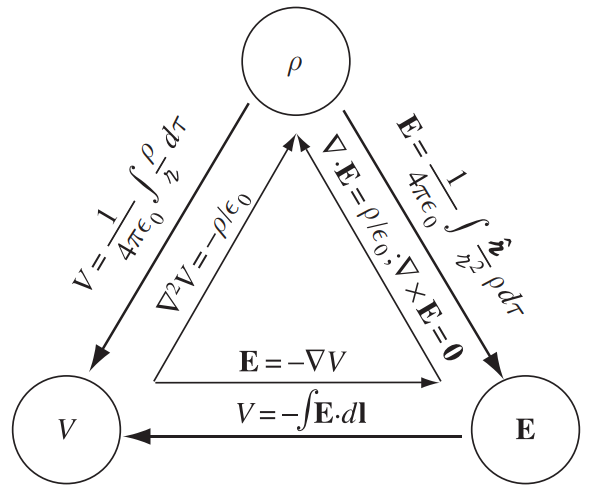
\includegraphics[width=0.7\textwidth]{Immagini/Relazioni.png} 
    \caption{Diagramma delle relazioni tra $\rho$, $V$ ed $\vec{E}$.}
    \label{fig:relazioni} 
\end{figure}

\chapter{Lavoro ed energia elettrostatica}

Supponiamo di avere una configurazione stazionaria di cariche e di voler spostare una carica \(Q\) dal punto \(a\) al punto \(b\) (supponendo che lo spostamento non perturb i il campo elettrostatico). Quanto lavoro si compie? In ogni punto lungo il percorso la forza che agisce su \(Q\) è la forza elettrica \(\vec{F}_{\rm campo}=Q\vec{E}\); la forza che si esercita in opposizione a questa forza elettrica, quando un agente esterno muove la carica lentamente, è \(\vec{F}_{\rm ext}=-Q\vec{E}\) (analoga al sollevare un mattone: la gravità esercita una forza \(mg\) verso il basso, mentre chi solleva esercita una forza \(mg\) verso l'alto).

La forza elettrostatica è conservativa, quindi il lavoro dipende solo dai punti iniziale e finale e non dal percorso.

\paragraph{Lavoro compiuto dal campo}
\[
W_{\rm campo}=\int_{a}^{b}\vec{F}_{\rm campo}\cdot d\vec{l}
=Q\int_{a}^{b}\vec{E}\cdot d\vec{l}
=-Q\bigl[V(b)-V(a)\bigr]
= -\Delta U,
\]
dove definiamo \(\Delta U=U(b)-U(a)\) come la variazione di energia potenziale elettrostatica.

\paragraph{Lavoro compiuto dall'agente esterno (quasi-statico)} 
\[
W_{\rm ext}=\int_{a}^{b}\vec{F}_{\rm ext}\cdot d\vec{l}
=-Q\int_{a}^{b}\vec{E}\cdot d\mathbf{l}
=Q\bigl[V(b)-V(a)\bigr]=\Delta U.
\]

Quindi si trovano i seguenti risultati:

\[
\boxed{\Delta U = Q\bigl[V(b)-V(a)\bigr] \qquad\text{e}\qquad
W_{\rm campo}=-\Delta U,\quad W_{\rm ext}=\Delta U.}
\]
\\
Se scegliamo il riferimento del potenziale in modo che \(V(\infty)=0\), il lavoro necessario (dall'agente esterno) per portare la carica \(Q\)
dall'infinito al punto \(\vec{r}\) è
\[
W_{\rm ext} = \Delta U = U(\vec{r})-U(\infty)=Q\bigl[V(\vec{r})-0\bigr]=Q\,V(\vec{r}).
\]
Si osserva che in questo caso il potenziale elettrico \(V\) è l'energia potenziale per unità di carica.

Si osserva che in questo caso il potenziale elettrico \(V\) è l'energia potenziale per unità di carica.
\section{Energia di un sistema discreto di cariche}
\section{Energia di un sistema con distribuzione continua di carica}
\section{Esempi}

\chapter{Materiali conduttori e isolanti}
\section{Campo elettrico in un materiale conduttore}
\section{Capacit\`a e condensatori}
\subsection{Condensatore all'infinito}
\section{Energia immagazzinata in un condensatore}
\section{Condensatore piano}
\section{Condensatore sferico}
\section{Condensatore cilindrico}

\chapter{I dipoli elettrici}
\section{Potenziale e campo elettrico di dipolo}
\section{Momento di dipolo di un sistema}
\section{Interazioni di dipolo in un campo elettrico di stimolo}
\section{Forza ed energia elettrostatica}
\subsection{Interazione dipolo-carica}
\subsection{Interazioni tra due dipoli}

\chapter{Correnti elettriche e campo di polarizzazione}
\section{La densit\`a di corrente elettrica}
\section{La corrente}
\section{Legge di conservazione della carica}
\subsection{Modelliziamo l'atomo}
\section{Carica elettrica legata e libera}
\section{Campo di polarizzazione}
\section{Densit\`a di carica superficiale nei materiali}
\section{La pila di volta}
\section{Potenza elettrica}
\section{Leggi di Ohm}
\subsection{Legge di Ohm locale}
\subsection{Legge di Ohm (macroscopica)}

\chapter{Campi elettrici nei materiali}
\section{Gabbia di Faraday}
\section{Condensatori in serie e parallelo}
\subsection{In serie}
\subsection{In parallelo}
\section{Campo di spostamento dielettrico}
\section{Relazione costitutiva interna}
\section{Condensatori reali}

\subsection{Condensatore piano con dielettrico}











\subsection{Considerazioni}




Notiamo che se $\varepsilon_0 >> 1$, allora $\sigma_f \sim \sigma_b$

\subsection{Condensatore piano con conduttore}
Inseriamo nel condensatore un conduttore, ma non a contatto con le armature, allora posso vederlo come più condensatori in serie
La capacità sarà quindi:


$$
C = \frac{\varepsilon_0 A}{d-b}
$$






\section{Esempi}

\subsection*{Esempio 1: dielettrici in serie}

Consideriamo un condensatore piano le cui armature hanno area \(A\) e in cui sono inseriti, in serie lungo la direzione del campo, due strati dielettrici di spessori \(h_1\) e \(h_2\) e costanti dielettriche relative \(\varepsilon_1\) e \(\varepsilon_2\). La differenza di potenziale tra le armature è \(V\). Assumendo campi uniformi e perpendicolari alle superfici, si può scrivere
\[
V = h_1 E_1 + h_2 E_2,
\]
dove \(E_1\) ed \(E_2\) sono i moduli dei campi elettrici nei due materiali.

Se sull'interfaccia non sono presenti cariche libere ($-\sigma_{{f}_{1}}+ \sigma_{{f}_{2}} = 0$), la componente normale del vettore \(\vec{D}\) è continua:
\[
D_{\perp1} = D_{\perp2} = D,
\]
ovvero, \(D\) è lo stesso in entrambi gli strati. Poiché \(\vec{D}=\varepsilon_0\varepsilon\,\vec{E}\), si ottiene
\[
E_1 = \frac{D}{\varepsilon_0\varepsilon_1},\qquad
E_2 = \frac{D}{\varepsilon_0\varepsilon_2}.
\]

Sostituendo in \(V\):
\[
V = D\left(\frac{h_1}{\varepsilon_0\varepsilon_1}+\frac{h_2}{\varepsilon_0\varepsilon_2}\right).
\]
Poiché il campo di spostamento è dato da \(D = \dfrac{Q}{A}\) (con \(Q\) carica sulle armature), risulta
\[
V = \frac{Q}{A}\left(\frac{h_1}{\varepsilon_0\varepsilon_1}+\frac{h_2}{\varepsilon_0\varepsilon_2}\right)
= Q\left(\frac{1}{\varepsilon_0 A}\left(\frac{h_1}{\varepsilon_1}+\frac{h_2}{\varepsilon_2}\right)\right).
\]
Dunque la capacità totale \(C\) del sistema è
\[
C=\frac{Q}{V}=\frac{\varepsilon_0 A}{\dfrac{h_1}{\varepsilon_1}+\dfrac{h_2}{\varepsilon_2}}.
\]

Introducendo le capacità dei singoli strati, \(C_1=\dfrac{\varepsilon_0\varepsilon_1 A}{h_1}\) e \(C_2=\dfrac{\varepsilon_0\varepsilon_2 A}{h_2}\), si ottiene la nota relazione per condensatori in serie:
\[
\frac{1}{C}=\frac{1}{C_1}+\frac{1}{C_2}.
\]

\subsection*{Esempio 2: dielettrici in parallelo}

Consideriamo ora due dielettrici affiancati (ad esempio due rettangoli contigui) inseriti fra le armature di un condensatore piano. Le armature sono equipotenziali e la differenza di potenziale tra di esse è \(V\); lo spessore comune dei dielettrici è \(h\). Poiché lo stesso potenziale viene applicato alle due regioni, il campo elettrico è lo stesso in entrambe:
\[
E=\frac{V}{h}.
\]

Tuttavia i materiali si polarizzano in modo diverso, quindi il vettore di spostamento normale \(\vec{D}_{\perp}\) è diverso nei due dielettrici:
\[
\vec{D}_{\perp,i}=\varepsilon_0\varepsilon_i\,\vec{E},\qquad i=1,2.
\]

La carica totale sulle armature è la somma delle cariche accumulate sopra ciascuna area \(A_1\) e \(A_2\):
\[
Q=Q_1+Q_2 = \vec{D}_{\perp,1}A_1 + \vec{D}_{\perp,2}A_2.
\]
Sostituendo \(\vec{D}_{\perp,i}=\varepsilon_0\varepsilon_i \vec{E}\) e \(E=V/h\) si ottiene
\[
Q = \varepsilon_0\frac{V}{h}\bigl(\varepsilon_1 A_1 + \varepsilon_2 A_2\bigr)
= V\underbrace{\frac{\varepsilon_0}{h}\bigl(\varepsilon_1 A_1 + \varepsilon_2 A_2\bigr)}_{C}.
\]
Quindi la capacità totale è
\[
C=\frac{\varepsilon_0}{h}\bigl(\varepsilon_1 A_1 + \varepsilon_2 A_2\bigr).
\]
Definendo le capacità dei singoli “rami” come \(C_i=\dfrac{\varepsilon_0\varepsilon_i A_i}{h}\), si verifica la legge dei condensatori in parallelo:
\[
C = C_1 + C_2.
\]

 
\section{Interfaccia vuoto -- dielettrico}

Vediamo cosa succede ai campi elettrici nell'interfaccia tra il vuoto e un materiale dielettrico.  
Indicheremo con \(\hat{n}\) il versore normale alla superficie (direzione convenzionale dal vuoto verso il dielettrico) e con \(\alpha\) l'angolo che il vettore campo forma con la \emph{superficie} (cioè con l'interfaccia).

Nel vuoto vale
\[
\vec{D}_{\mathrm{est}}=\varepsilon_0\vec{E}_{\mathrm{est}},
\]
mentre nel dielettrico 
\[
\vec{D}_{\mathrm{int}}=\varepsilon_0\varepsilon\,\vec{E}_{\mathrm{int}}.
\]

\noindent{\bf Condizioni al contorno sull'interfaccia vuoto--dielettrico.}  
Se indichiamo con \(\alpha_{\text{est}}\) e \(\alpha_{\text{int}}\) gli angoli di \(\vec{E}_{\text{est}}\) e \(\vec{E}_{\text{int}}\) rispetto all'interfaccia, allora le componenti parallela e perpendicolare di \(\vec{E}\) si esprimono come
\[
E_{\parallel}=E\cos\alpha,\qquad E_{\perp}=E\sin\alpha.
\]

\begin{itemize}
  \item la componente parallela di \(\vec{E}\) è continua (si conserva):
  \[
  \vec{E}_{\mathrm{est},\parallel}=\vec{E}_{\mathrm{int},\parallel},
  \]
  che in forma scalare diventa
  \[
  E_{\mathrm{est}}\cos\alpha_{\mathrm{est}} = E_{\mathrm{int}}\cos\alpha_{\mathrm{int}}.
  \]

  \item la componente perpendicolare di \(\vec{D}\) presenta una discontinuità (non si conserva) pari alla densità di carica libera sulla superficie \(\sigma_{\mathrm{f}}\):
  \[
  \vec{D}_{\mathrm{est},\perp}-\vec{D}_{\mathrm{int},\perp}=\sigma_{\mathrm{f}}.
  \]
  In assenza di carica libera sulla superficie (\(\sigma_{\mathrm{f}}=0\)) si ha quindi
  \[
  \vec{D}_{\mathrm{est},\perp}=\vec{D}_{\mathrm{int},\perp},
  \]
  che in forma scalare diventa
  \[
  D_{\mathrm{est}}\sin\alpha_{\mathrm{est}} = D_{\mathrm{int}}\sin\alpha_{\mathrm{int}}.
  \]
\end{itemize}
\vspace{0.2cm}
Ora sostituiamo \(D_{\mathrm{est}}=\varepsilon_0 E_{\mathrm{est}}\) (vuoto) e \(D_{\mathrm{int}}=\varepsilon_0\varepsilon E_{\mathrm{int}}\) (dielettrico) nella condizione sulla componente perpendicolare:
\[
\varepsilon_0 E_{\mathrm{est}}\sin\alpha_{\mathrm{est}}
= \varepsilon_0\varepsilon\,E_{\mathrm{int}}\sin\alpha_{\mathrm{int}}
\quad\Longrightarrow\quad
E_{\mathrm{est}}\sin\alpha_{\mathrm{est}} = \varepsilon\,E_{\mathrm{int}}\sin\alpha_{\mathrm{int}}.
\]

Infine facendo il rapporto si trova:

\[
\frac{E_{\mathrm{est}}\sin\alpha_{\mathrm{est}}}{E_{\mathrm{est}}\cos\alpha_{\mathrm{est}}}
= \frac{\varepsilon\,E_{\mathrm{int}}\sin\alpha_{\mathrm{int}}}{E_{\mathrm{int}}\cos\alpha_{\mathrm{int}}}.
\]

ottenendo
\[
\boxed{\;\tan\alpha_{\mathrm{est}}=\varepsilon\,\tan\alpha_{\mathrm{int}}\; }.
\]

\noindent{\bf Interpretazione e casi limite}

\begin{itemize}
\item{La componente perpendicolare di \(\vec{E}\)  in generale non è continua (non si conserva): la sua discontinuità è causata dalle cariche sulla superficie (libere o legate). 
\[
\vec{D}=\varepsilon_0\vec{E}+\vec{P},
\]
Può risultare meno intuitivo che la componente parallela di \(\vec{D}\) non sia necessariamente continua. In elettrostatica si ha \(\nabla\times\vec{E}=0\), perciò \(\vec{E}_{\parallel}\) è continuo; invece
\[
\nabla\times\vec{D}=\nabla\times\vec{P},
\]
quindi se la polarizzazione \(\vec{P}\) ha rotore non nullo allora \(\nabla\times\vec{D}\neq 0\) e la componente parallela di \(\vec{D}\) può essere discontinua.}

  \item Se $\varepsilon>1$, allora $\tan\alpha_{\text{int}}>\tan\alpha_{\text{est}}$, cioè $\alpha_{\text{int}}>\alpha_{\text{est}}$: all'interno del dielettrico il campo si inclina maggiormente rispetto alla normale e quindi risulta più parallelo all'interfaccia.
  \item Per incidenza perpendicolare ($\alpha_{\text{est}}=0$) si ha $\alpha_{\text{int}}=0$ (non c'è deviazione).
  \item Nel limite $\varepsilon\to\infty$ si ottiene $\alpha_{\text{int}}\to 90^\circ$ (campo quasi parallelo all'interfaccia).
\end{itemize}


\section{Problema di Dirichlet}

Consideriamo una disposizione di pezzi di rame (conduttori), ciascuno collegato tramite fili di rame al polo di una propria batteria. Gli altri poli delle batterie sono collegati mediante fili alla parete di una gabbia di Faraday in rame, che fa da massa (potenziale di riferimento, scelto uguale a zero).

Quando le correnti cessano (regime elettrostatico), la condizione di equilibrio ( o dalla legge di Ohm si) impone che ogni conduttore sia equipotenziale: cioè ciascun pezzo di rame assume un potenziale costante su tutta la sua superficie.

\medskip

\noindent\textbf{Problema di Dirichlet.} Determinare il potenziale elettrico \(V(\vec r)\) nella regione dello spazio esterna ai conduttori, imponendo che \(V\) assuma i valori assegnati sulle superfici dei conduttori e che sia nullo sulla massa (gabbia di Faraday).
\\
\\
Per ottenere il campo elettrico si calcola \(\vec{E}(\vec r)=-\nabla V(\vec r)\). Nella regione esterna ai conduttori le cariche libere sono distribuite solo sulle superfici dei conduttori stessi: Nello spazio compreso fra le superfici dei conduttori e le pareti della gabbia non è presente una densità di carica volumetrica libera. Di conseguenza l'equazione di Poisson
\[
\nabla^2 V(\vec r) = -\frac{\rho(\vec r)}{\varepsilon_0}
\]
si riduce all'equazione di Laplace
\[
\nabla^2 V(\vec r)=0
\]
nel dominio considerato (regione esterna ai conduttori e interna alla gabbia), soggetta alle condizioni al contorno di Dirichlet sopra specificate.


\chapter{Interazioni e campi di risposta}
\section{Interazione carica-carica indotta}
\subsection{Caso limite}
\subsection{Applicazione}
\section{Interazione carica-dipolo indotto}
\subsection{In generale}
\section{Sfere con distribuzione di carica opposta}
\section{Polarizzazione di una sfera dielettrica}

\chapter{Magnetismo}
\section{Introduzione}
\section{Legge di Biot--Savart}
\section{II equazione di Maxwell}
\section{Forza di Lorentz}
\section{Campo di magnetizzazione}
\subsection{Interpretazione}
\section{Esempi}

\chapter{Legge di Ampere-Maxwell e campo magnetico H}
\section{IV equazione di Maxwell}
\section{Teorema di equivalenza di Amp\`ere}
\section{Esempi}

\chapter{Potenziale vettore di Amp\`ere}
\section{Esempi}
\section{Legge di Biot--Savart}
\section{Esempi aggiuntivi}
\section{Interazioni magnetiche}

\chapter{Come i materiali reagiscono ai campi magnetici di stimolo}
\section{Relazione costitutiva interna}
\section{Misure di suscettivit\`a magnetica}

\chapter{Strumenti e applicazioni}
\section{Amperometro}
\subsection{Misure stazionarie di conducibilit\`a}
\section{Modello a tempo di rilassamento}
\section{Effetto Hall}
\section{Effetto Joule}
\section{Leggi di Kirchhoff}
\section{Circuito RC ed energia dissipata}
\section{Studio dei condensatori con dielettrico}
\subsection{Densit\`a di energia elettrica}
\subsection{Forze che agiscono sul dielettrico}

\chapter{Introduzione all'elettrodinamica}
\section{Forza di Lorentz e moti di ciclotrone}
\section{Relativit\`a del campo elettrico}
\section{Legge di induzione}
\section{III legge di Maxwell}
\section{Esempi}
\section{Forze magnetodinamiche}
\subsection{Esempi}
\section{Alternatore--Generatore di corrente monofase}

\chapter{Induttanza e circuiti}
\section{Induttanza}
\section{Densit\`a di energia magnetica}
\section{Circuiti RCL in serie in regime transitorio}
\section{Circuiti RCL in regime armonico}
\subsection{Curva di risonanza di un circuito RCL}

\chapter{Materiali ferromagnetici}
\section{Legge di Felici}
\section{Ciclo di isteresi}
\section{Magneti permanenti}
\section{Campi magnetici nei materiali lineari}
\section{Interfaccia tra due materiali lineari}
\section{Esempi}
\section{Circuiti magnetici}
\section{Trasformatore}







\end{document}
